\chapter{Deriving Rules}
\label{sec:rules}

The identification of useless mutants is important to support developers on deriving rules to avoid the generation of such mutants. 
To derive the rules, we manually analyzed a total of 2,345 programs (50 programs + 963 equivalent mutants + 1,332 duplicated mutants). 
In this chapter, we first define what is a rule and then we illustrate several examples of rules we derived from the results of executing our strategy.


\section{Rule to Avoid Useless Mutants}
\label{sec:rules-definition}

To avoid the generation of these mutants, we develop rules.
A rule to avoid useless mutants is defined as a triple $(terms,~ transformations,~constraints)$, where:

\begin{itemize}
	
	\item \textit{term} is any Java language construct;
	
	\item \textit{transformations} is a set of mutation operators applied to \textit{term} or to one of its subterms; and
	
	\item \textit{constraints} is a set of conditions on $term$ or on the arguments of the mutation operators in $transformations$ that guarantee that the rule indeed avoids useless mutants.
	
\end{itemize}


In this context, \textit{term} represents the language constructs to which the \textit{transformations} (the mutations) will be applied. 
A rule to avoid an equivalent mutant (E-Rule) states that no mutation operator in \textit{transformation} should be applied whatsoever. 
On the other hand, a rule to avoid a duplicated mutant (D-Rule) states that only one of the mutation operators in \textit{transformations} should be applied. 
In this sense, by applying our rules right before the mutants generation, we can avoid useless mutants. 
To better explain the \textit{transformations} we use in our rules, we refer to the meta-variables presented in Table~\ref{tab:meta-variables}.

\scriptsize
\begin{table}[ht]
	\centering
	\caption{Meta-variables referred by the rules.}
	\label{tab:meta-variables}
	\begin{tabular}{|c|l|}
		\hline
		\textbf{Meta-variables} & \multicolumn{1}{c|}{\textbf{Description}} \\ \hline
		$op$         & any binary or unary operator \\ \hline
		$exp$        & any expression \\ \hline
		$b$          & any block of statements \\ \hline
		$s$          & any statement \\ \hline
		$;$          & an empty statement \\ \hline
		$C, D$          & class references \\ \hline
		$v$          & \begin{tabular}[c]{@{}l@{}}any identifier of variable, array access, or field \\ access for a primitive integral type (byte, short, int, long)\end{tabular} \\ \hline
	\end{tabular}
\end{table}
\normalsize

%Table~\ref{tab:mutationoperators} presents examples of \textit{transformations} performed by some mutation operators. 
%Notice that one operator may have more than one transformation, such as the ROR operator (Relational Operator Replacement).

Table~\ref{tab:mutationoperators} presents examples of \textit{transformations} performed by some mutation operators. 
For example, the LOI operator (Logical Operator Insertion) receives $v$ as input---see this meta-variable in Table~\ref{tab:meta-variables}---and returns $\sim v$. 
Mutation operators can also delete an entire statement. 
For instance, the SDL operator (Statement Deletion) deletes a given statement $s$, i.e., $SDL(s) =~;$~. 
The ROR operator (Relational Operator Replacement) has more than one transformation. 
The first and second transformations (ROR$_1$ and ROR$_2$) replace an entire expression by \texttt{false} and \texttt{true}, respectively. 
The third one (ROR$_3$) takes two binary operators as input, i.e., $op_1$ and $op_2$. 
Then, the operator replaces the first ($op_1$) by the second ($op_2$), as long as $op_1$ and $op_2$ $\in$ \{>, >=, <, <=, ==, !=\} and $op_1~\neq~op_2$.



%\scriptsize
\begin{table}[t]
	\centering
	\caption{Examples of transformations performed by some mutation operators. This table contains only a subset of all possible transformations performed by the mutation operators.}
	\label{tab:mutationoperators}
	\resizebox{\textwidth}{!}{%
	\begin{tabular}{|c|l|l|}
		\hline
		\textbf{Mutation Operators}                                                                        & \multicolumn{1}{c|}{\textbf{Transformations}}                                                                                                                                                                  & \multicolumn{1}{c|}{\textbf{Tool}} \\ \hline
		\begin{tabular}[c]{@{}c@{}}LOI \\ (Logical Operator Insertion)\end{tabular}                        & $LOI(v)~=~\sim~v$                                                                                                                                                                                           & \mujava{}                             \\ \hline
		\begin{tabular}[c]{@{}c@{}}LOD \\ (Logical Operator Deletion)\end{tabular}                         & $LOD(\sim~exp)$ = $exp$                                                                                                                                                                                           & \mujava{}                             \\ \hline
		\begin{tabular}[c]{@{}c@{}}ODL \\ (Operator Deletion)\end{tabular}                                 & \begin{tabular}[c]{@{}l@{}}$ODL_1(exp_1~op~exp_2) = exp_1$\\ $ODL_2(exp_1~op~exp_2) = exp_2$\end{tabular}                                                                                                                  & \mujava{}                             \\ \hline
		\begin{tabular}[c]{@{}c@{}}VDL \\ (Variable Deletion)\end{tabular}                                 & $VDL(v~op~exp) = exp$                                                                                                                                                                                            & \mujava{}                             \\ \hline
		\begin{tabular}[c]{@{}c@{}}AOIU \\ (Arithmetic Operator Insertion)\end{tabular}                                 & $AOIU(v) = -v$                                                                                                                                                                                            & \mujava{}                             \\ \hline
		\begin{tabular}[c]{@{}c@{}}AODU \\ (Arithmetic Operator Deletion)\end{tabular}                                 & $AODU(-exp) = exp$                                                                                                                                                                                            & \mujava{}                             \\ \hline
		\begin{tabular}[c]{@{}c@{}}ROR \\ (Relational Operator Replacement)\end{tabular}                   & \begin{tabular}[c]{@{}l@{}} $ROR_1(exp_1~op~exp_2) = false,~if~op~ \in~\{>,~>=,~<,~<=,~==,~!=\}$\\ 
			$ROR_2(exp_1~op~exp_2) = true,~if~op~ \in~\{>,~>=,~<,~<=,~==,~!=\}$\\ 
			$ROR_3(op_1,~op_2) = op_2,~if~op_1,~op_2~ \in~\{>,~>=,~<,~<=,~==,~!=\}~and~op_1~ \neq ~op_2$ \end{tabular} & \mujava{}                             \\ \hline
		\begin{tabular}[c]{@{}c@{}}SDL \\ (Statement Deletion)\end{tabular}                                & $SDL(s) =  $~$;$                                                                                                                                                                                                     & \mujava{}                             \\ \hline
		\begin{tabular}[c]{@{}c@{}}ISD \\ (super keyword deletion)\end{tabular}                            & $ISD(super.v) = v$                                                                                                                                                                                               & \mujava{}                             \\ \hline
		\begin{tabular}[c]{@{}c@{}}PNC \\ (new method call with child class type)\end{tabular}                            & $PNC(C, D) = D$                                                                                                                                                                                               & \mujava{}                             \\ \hline
		
		\begin{tabular}[c]{@{}c@{}}AOR \\ (Arithmetic Operator Replacement)\end{tabular}                   & $AOR(op_1,~op_2)~=~op_2, if~op_1,~op_2~\in~\{+,-,*,/,\%\}~$and$~op_1 \neq op_2$                                                                                                                                              & \major{}                              \\ \hline
		\begin{tabular}[c]{@{}c@{}}LVR \\ (Literal Value Replacement)\end{tabular}                         & \begin{tabular}[c]{@{}l@{}}$LVR(1) = 0$\\ $LVR(0) = 1$\end{tabular}                                                                                                                                                & \major{}                              \\ \hline
		\begin{tabular}[c]{@{}c@{}}InlineConstant \\ (Replaces inline constants)\end{tabular}               & \begin{tabular}[c]{@{}l@{}}$InlineConstant(1) = 0$\\ $InlineConstant(-1) = 1$\end{tabular}                                                                                                                         & \pit{}                                \\ \hline
		\begin{tabular}[c]{@{}c@{}}RemoveConditionals \\ (Replaces conditionals)\end{tabular} & $RemoveConditionals(exp) = false$                                                                                                                                                                  & \pit{}                                \\ \hline
		\end{tabular}
	}
\end{table}
%\normalsize

As an example, we now present a rule to detect an equivalent mutant. The ISD operator (super keyword deletion) deletes the \texttt{super} keyword from the $super.v$ term. In case $v$ exists only in the superclasses, the rule would prevent the mutation testing tool from applying the mutation operator in \textit{transformations}, i.e., the ISD operator, avoiding an equivalent mutant.
\\
\\
\textbf{E-Rule. ISD}\\
$term = super.v$\\
$transformations = \{\\ \indent ISD(super.v) =~v \\\}$\\
$constraints = \{ \\ \indent v$~exists~only~in~superclasses \\ $\}$\\

The aforementioned rule has been presented elsewhere~\cite{OFFUT:2006:1}. In the next section, we present a subset of the new rules we have identified.

\section{Examples of Rules}
\label{sec:examples-of-rules}

To better explain the rules we identified, we refer to six code snippets generated by our strategy presented in Figure~\ref{fig:useless-examples} (a--f). 
The left-hand side represents a code snippet from the original program. 
We underline the \textit{terms} to be transformed (mutated). 
To present examples of equivalents and duplicated mutants, we use two and three boxes, respectively. 
We present the mutation operators at the top of the boxes.

%\begin{figure*}[ht]
%	\begin{center}
%		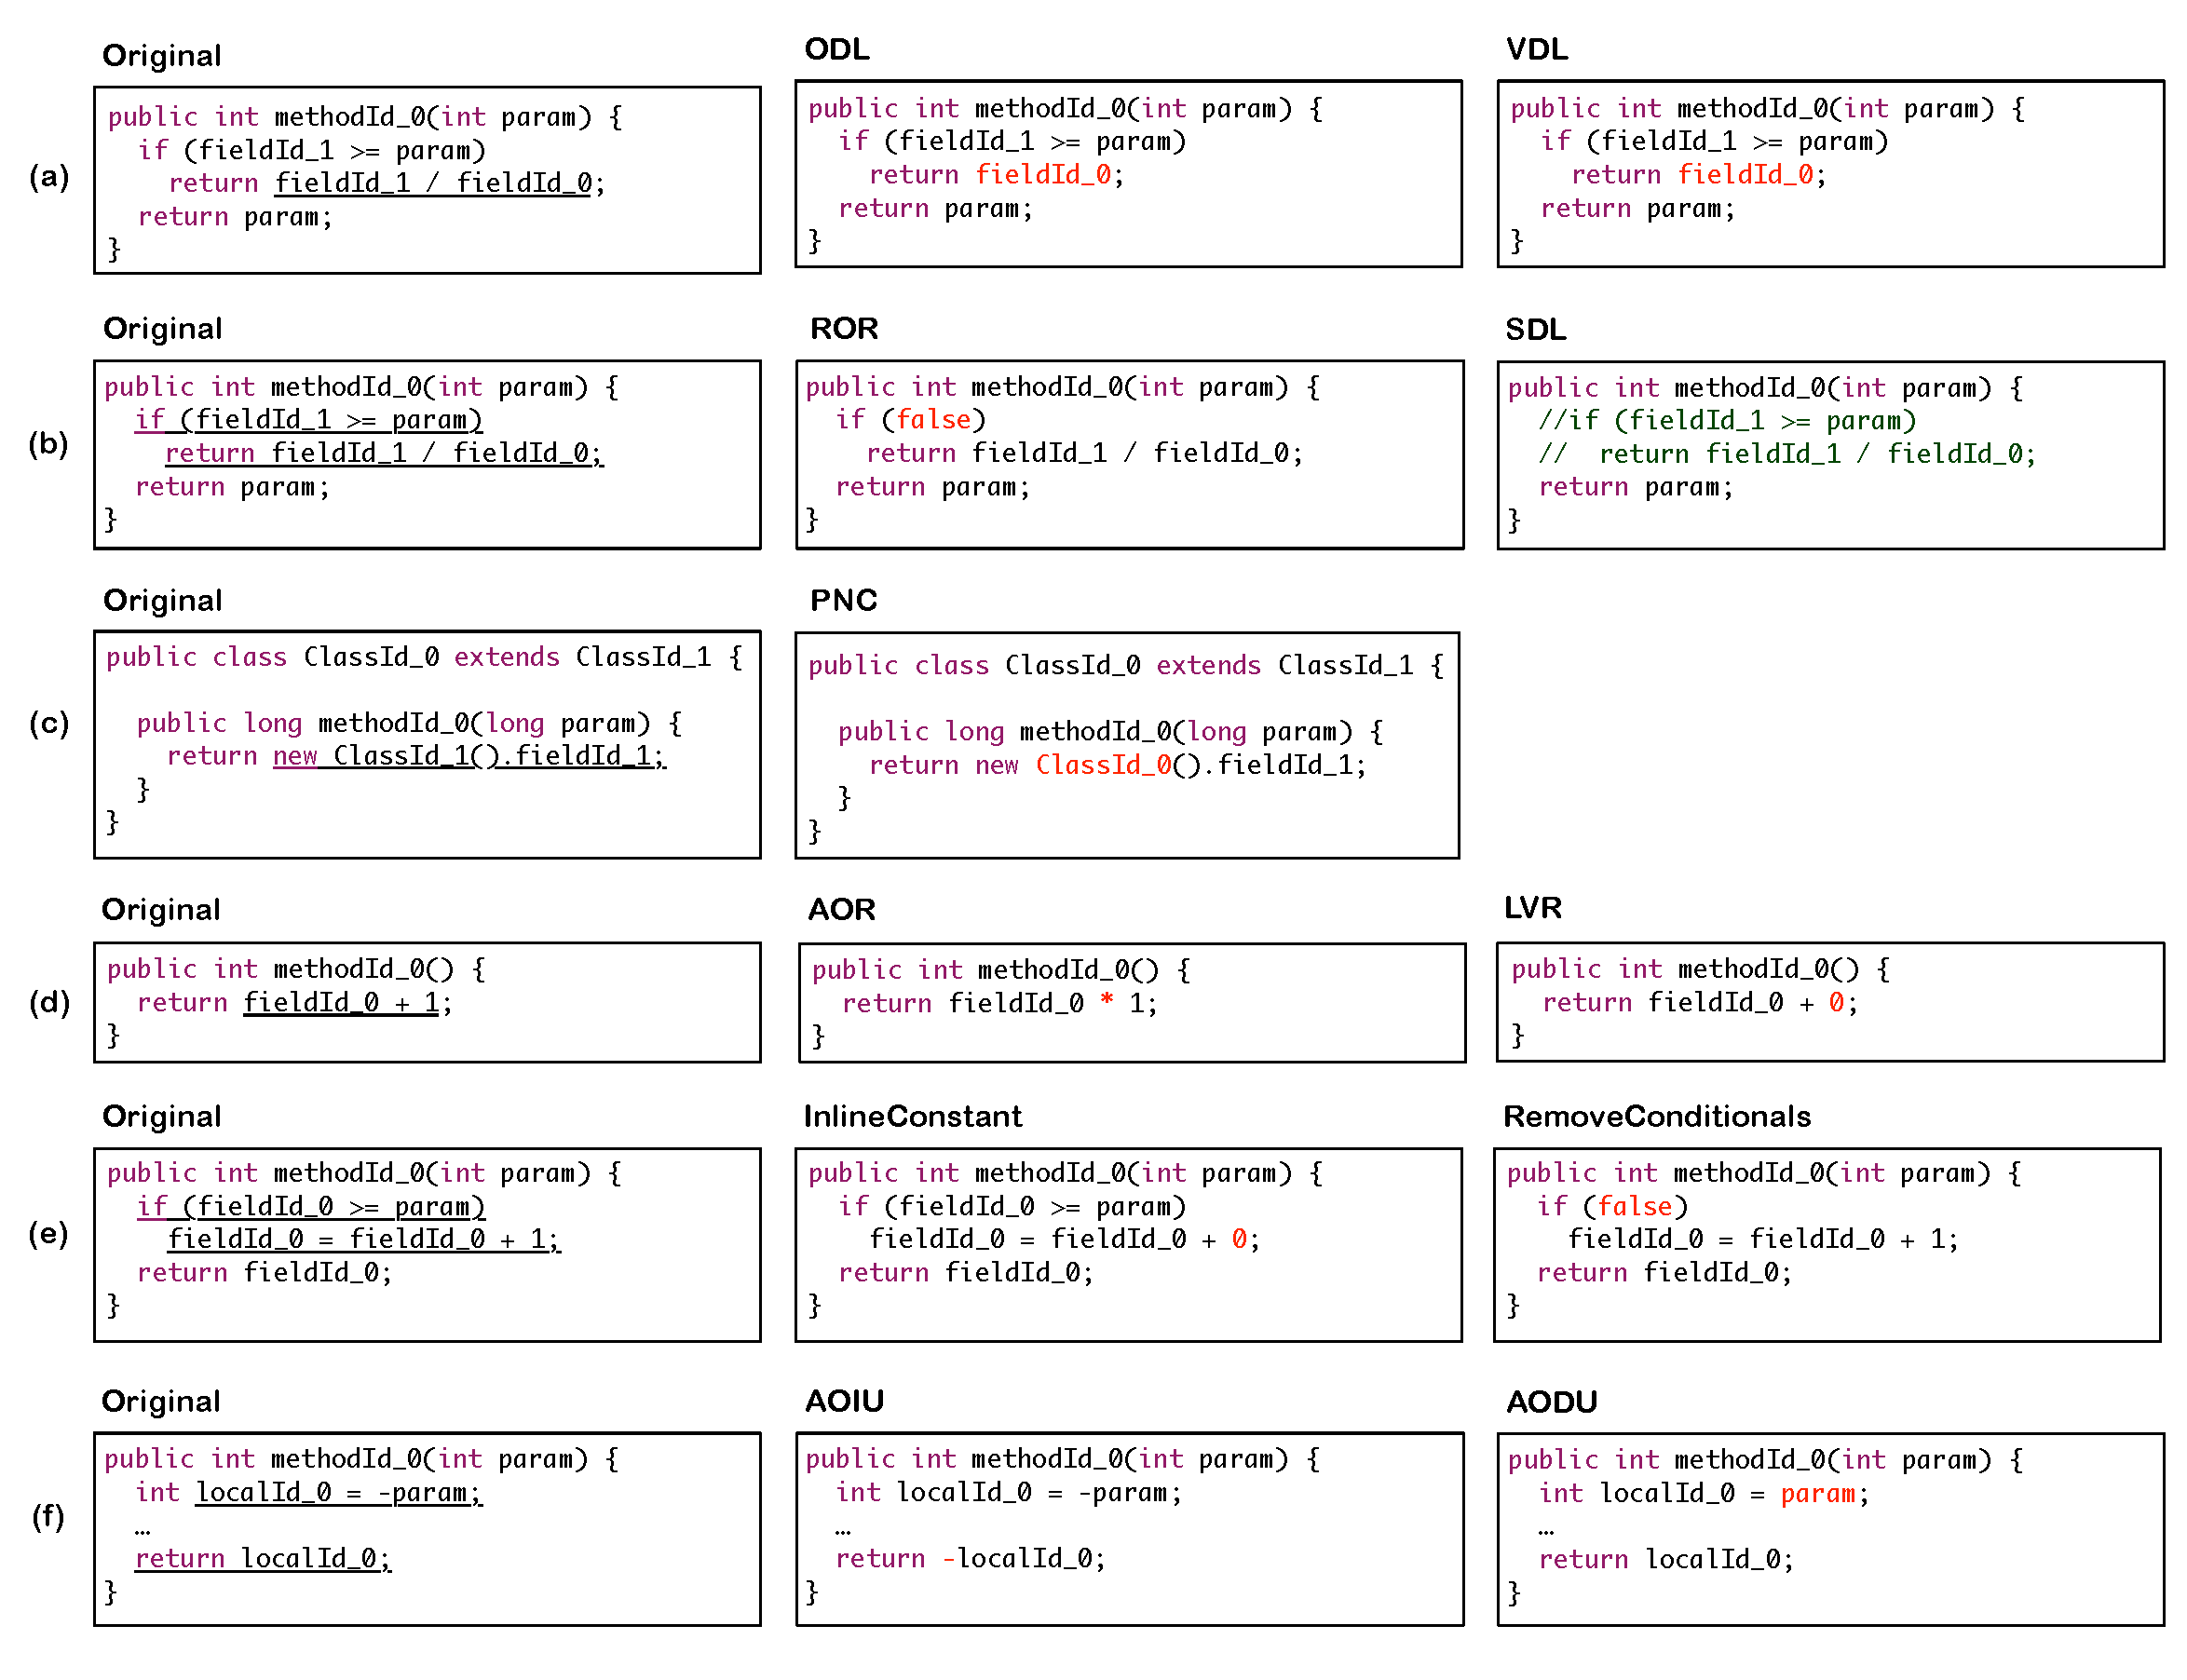
\includegraphics[scale=0.37]{images/Useless-Examples.pdf}
%		\caption{Original programs generated by \jdolly{} and useless mutants examples.}
%		\label{fig:useless-examples}
%	\end{center}
%\end{figure*}

\begin{figure*}[ht]
	\begin{center}
		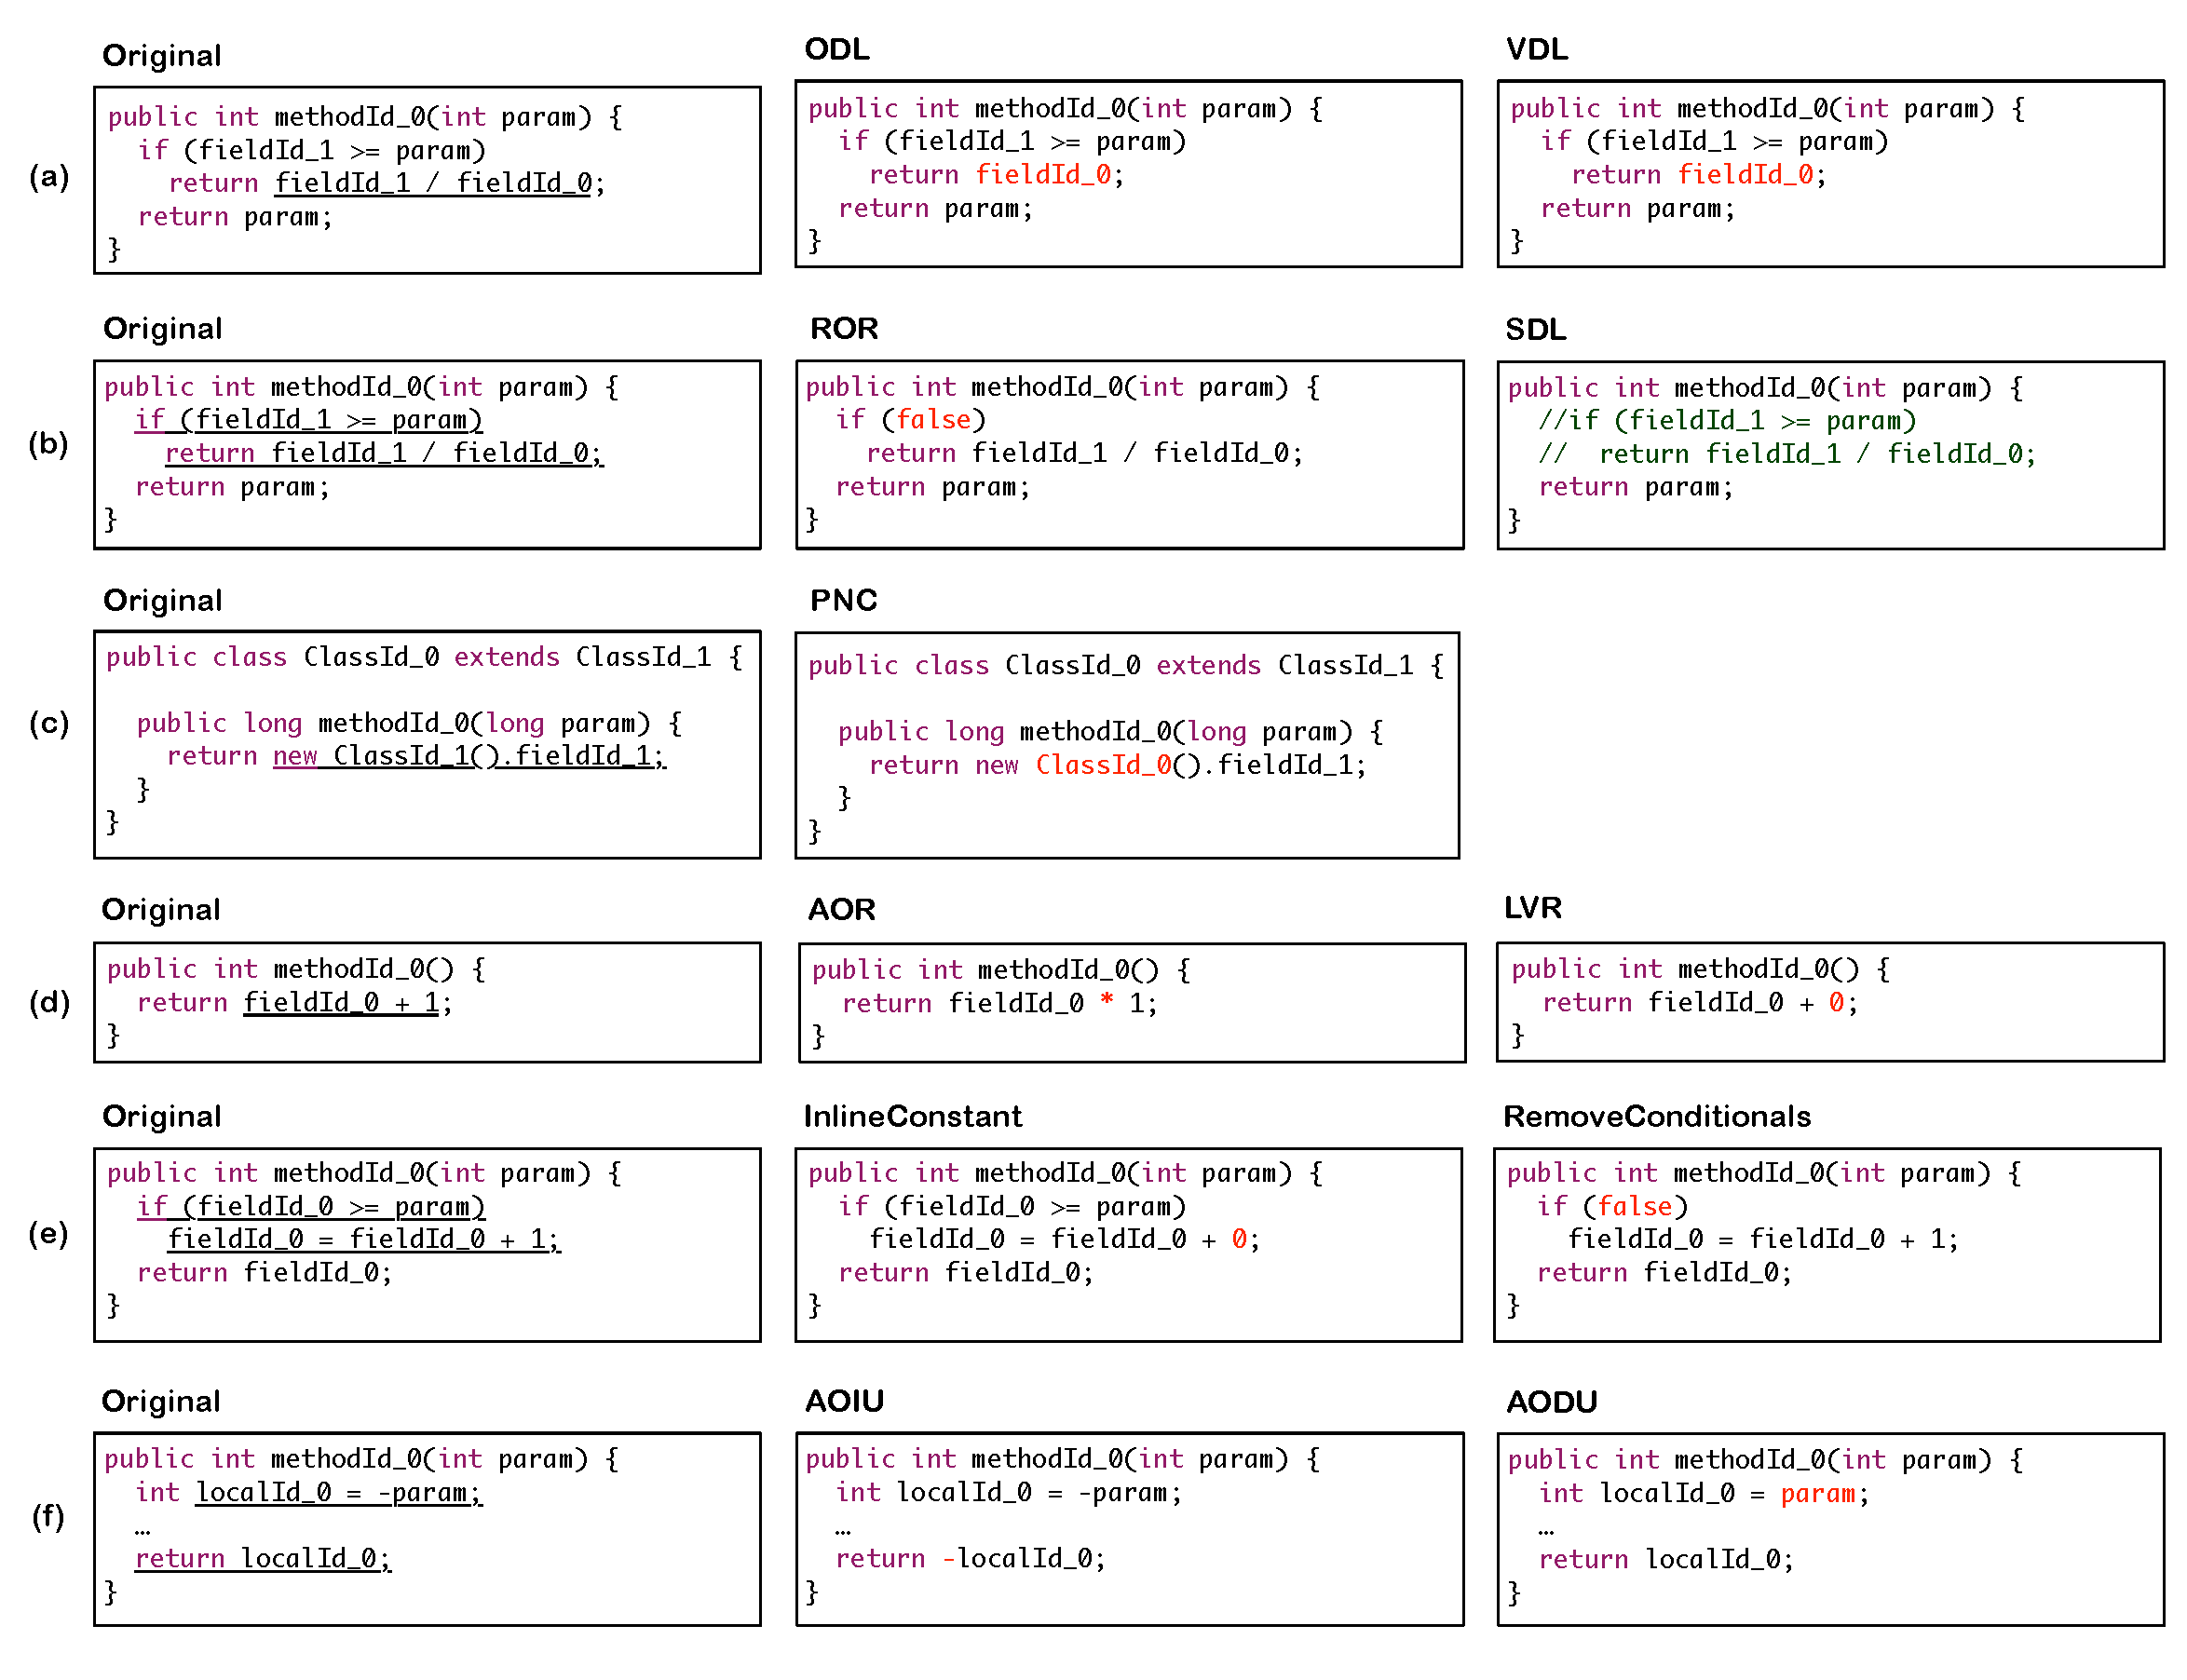
\includegraphics[scale=0.37]{images/Useless-Examples.pdf}
		\caption{Code snippets from programs generated by \jdolly{} and some of its useless mutants.}
		\label{fig:useless-examples}
	\end{center}
\end{figure*}

We now proceed as follows. Section~\ref{sec:no-def-use} presents rules that do not need \textit{def-use} analyses to be implemented. In contrast, Section~\ref{sec:def-use} presents rules that need \textit{def-use} analyses.

\subsection{Rules that do not need def-use analyses}
\label{sec:no-def-use}

Figure~\ref{fig:useless-examples}(a) illustrates an example of duplicated mutants with the exact same source code. These mutants have been generated by using the ODL and VDL operators (Operator and Variable Deletion). This way, according to the following rule, only one mutation operator in \textit{transformations} should be applied. The \textit{constraints} set is empty for this rule.
%We also identified a rule that can avoid the generation of mutants with the same exact source code. Figure~\ref{fig:useless-examples}(b) illustrates this case. The \mujava{} operators ODL and VDL (Operator and Variable Deletion) generated the same exact source code. This way, according to the following rule, only one mutation operator in \textit{transformations} should be applied. The \textit{constraints} set is empty for this rule.
\\
\\
\textbf{D-Rule. ODL x VDL}\\
$term = exp~op~v $\\
$transformations = \{\\ \indent ODL(exp~op~v) = exp,\\ \indent VDL(exp~op~v) = exp\\\}$\\

Figure~\ref{fig:useless-examples}(b) presents a code snippet that contains an \texttt{if} statement. Whilst the ROR operator (Relational Operator Replacement) sets the boolean expression to \texttt{false} (i.e., the \texttt{if} body will not be executed), the SDL operator (Statement Deletion) deletes the entire \texttt{if} statement. Therefore, these mutants are duplicated. We introduce a rule to identify this case as follows. Notice that the \textit{term} matches with an \texttt{if} statement without \texttt{else}. The \textit{constraints} set is empty.
%Figure~\ref{fig:useless-examples}(c) presents a program that contains an \texttt{if} statement. Whilst the ROR operator (Relational Operator Replacement) sets the boolean expression to \texttt{false} (i.e., the \texttt{if} body will not be executed), the SDL operator (Statement Deletion) deletes the entire \texttt{if} statement. Therefore, these mutants are duplicated. We introduce a rule to identify this case as follows. Notice that the \textit{term} matches with an \texttt{if} statement without \texttt{else}. The \textit{constraints} set is empty in this rule.
\\
\\
\textbf{D-Rule. ROR x SDL}\\
$term = if~(exp_1~op~exp_2)~\{b\} $\\
$transformations = \{\\ \indent ROR(exp_1~op~exp_2) = false, \\ \indent SDL(if~(exp_1~op~exp_2)~\{b\}) =~; \\ \}$\\

The next rule uses the bitwise complement operator ($\sim$), which simply flips bits (e.g., 00000010 becomes 11111101). To better explain this rule, consider that the original code contains a field with this operator (\texttt{$\sim$fieldId\_0}). In this context, when applying the \mujava{} operators LOI (Logical Operator Insertion) and LOD (Logical Operator Deletion) into the aforementioned field, we have duplicated mutants. In this example, LOI inserts the bitwise complement operator (\texttt{$\sim\sim$fieldId\_0}) and LOD removes (\texttt{fieldId\_0}). We define a rule to identify this case in what follows. In our rule, we apply LOI to the subterm $v$, not to the entire term $\sim$$v$. Notice that the \textit{constraints} set in this rule is empty.
%Figure~\ref{fig:useless-examples}(a) illustrates an example of duplicated mutants. Notice that the original code contains a field with a bitwise complement operator (\texttt{$\sim$fieldId\_0}). In this context, when applying the \mujava{} operators LOI (Logical Operator Insertion) and LOD (Logical Operator Deletion) into the aforementioned field, we have duplicated mutants (i.e., one of them is useless). In this example, LOI inserted the bitwise complement operator (\texttt{$\sim\sim$fieldId\_0}) and LOD removed (\texttt{fieldId\_0}). We define a rule to identify this case in what follows. In our rule, we apply LOI to the subterm $v$, not to the entire term $\sim$$v$. Notice that the \textit{constraints} set in this rule is empty.
\\
\\
\textbf{D-Rule. LOI x LOD}\\
$term = {\sim}v$\\
$transformations = \{\\ \indent LOI(v) = {\sim\sim} v,\\ \indent LOD({\sim}v) = v \\\}$\\

For the next rule, we avoid duplicated mutants that are generated by the same mutation operator. In the first mutant, the SDL operator (Statement Deletion) deletes the entire \texttt{if} statement; in the second one, it deletes the only statement within the \texttt{if} body. Notice that both mutants are duplicated, as long as \textit{constraints} hold: the \texttt{if} expression has no side effect. In this rule, \textit{term} matches with an \texttt{if} statement containing only one statement $s$ (refer to Table~\ref{tab:meta-variables}) without \texttt{else}.
%We also detected the same mutation operator generating duplicated mutants (see Figure~\ref{fig:useless-examples}(d)). In the first mutant, the SDL operator (Statement Deletion) deletes the entire \texttt{if} statement; in the second one, it deletes the only statement within the \texttt{if} body. Notice that both mutants are duplicated, as long as \textit{constraints} hold: the \texttt{if} expression has no side effect. In this rule, \textit{term} matches with an \texttt{if} statement containing only one statement $s$ (refer to Table~\ref{tab:meta-variables}) without \texttt{else}.
\\
\\
\textbf{D-Rule. SDL x SDL}\\
$term = if~(exp)~{~s~} $\\
$transformations = \{\\ \indent SDL(s) =~;, \\ \indent SDL(if~(exp)~s) =~; \\ \}$\\
$constraints = \{\\$ \indent $exp$~has~no~side~effect $\\\}$\\

%\todo{Esta regra nao necessita meso de def-use???}
We now present an E-Rule, i.e., a rule to identify equivalent mutants. We derived this rule by using a \mujava{} operator. Figure~\ref{fig:useless-examples}(c) shows a code example to better explain the rule. The PNC operator replaces superclass $C$ by subclass $D$. In this situation, field \texttt{v} must be declared only in $C$. In addition, the subclass constructor must not change \texttt{v} and calls the same superclass constructor defined in \textit{term}.
\\
\\
\textbf{E-Rule. PNC}\\
$term = new~C().v $\\
$transformations = \{ \\ \indent PNC(C, D)~=~D \\ \}$\\
$constraints = \{$ \\ \indent $D$~extends~$C$, \\ \indent $v$~exists only in$~C$, \\ \indent $D$~constructor does not change$~v$, \\ \indent $D$~constructor calls the same~$C$~constructor \\ \}$ $\\

The rules presented so far have been derived from mutation operators of \mujava{}. We now illustrate two rules derived by using \major{} and \pit{} operators. Figure~\ref{fig:useless-examples}(d) illustrates an example of duplicated mutants generated by \major{}. Notice that the original code contains the following binary expression: \texttt{fieldId\_0 + 1}. The AOR operator (Arithmetic Operator Replacement) replaces one operator by another. This way, AOR receives two operators as input in our rule, i.e., $op_1$ and $op_2$, and then replaces the first by the second. The LVR operator (Literal Value Replacement) replaces the literal one by the literal zero. In case we apply both mutation operators and \textit{constraints} hold, i.e., $op_1 \in \{+,-\}$ and $op_2 \in \{*,/\}$, we end up with duplicated mutants (e.g., \texttt{fieldId\_0 * 1} \textit{versus} \texttt{fieldId\_0 + 0}). We present a rule to avoid this situation in what follows.
\\
\\
\textbf{D-Rule. AOR x LVR}\\
$term =  exp~op_1~1 $\\
$transformations = \{ \\ \indent AOR(exp~op_1~1,~op_2) = exp~op_2~1, \\
\indent LVR(1)=0 \\ \}$\\
$constraints = \{\\ \indent op_1~\in~\{+, -\}~, \\ \indent op_2~\in~\{*, /\} \\ \}$\\

Now we present a rule we derived when using the \pit{} mutation testing tool. To better understand this rule, consider Figure~\ref{fig:useless-examples}(e). The InlineConstant operator replaced the literal one by the literal zero, yielding \texttt{fieldId\_0 = fieldId\_0 + 0;}. On the other hand, the RemoveConditionals operator changed the \texttt{if} expression to \texttt{false}. In this case, the first mutant does not change the \texttt{fieldId\_0} value. The second mutant does not change it as well, since the \texttt{if} body will not be executed. The rule to identify such case is presented in what follows. In this rule, notice that \textit{term} matches with an \texttt{if} statement containing only $v := v~op~1$ with no \texttt{else} statement.
\\
\\
\textbf{D-Rule. InlineConstant x RemoveConditionals}\\
$term = if~(exp)~{~v~:=~v~op~1} $\\
$transformations = \{ \\ \indent InlineConstant(1)~=~0,\\ \indent RemoveConditionals(exp)=false \\ \}$\\
$constraints = \{ \\$ \indent $op~\in~\{+, -\}$, \\ \indent $exp$~has~no~side~effect $ \\ \}$

\subsection{Rules that need def-use analyses}
\label{sec:def-use}

Using only the Abstract Syntax Tree (AST) is not enough to implement some of the rules we have identified. They need \textit{def-use} analyses. We now present a rule for this case. Whilst the AODU operator (Arithmetic Operator Deletion) removes the minus operator from the statement \texttt{localId\_0 = -param;}, the AOIU operator (Arithmetic Operator Insertion) inserts the minus at the \texttt{return} statement (\texttt{return -localId\_0;}). To better understand this rule, consider the code snippet presented in Figure~\ref{fig:useless-examples}(f). In this situation, one constraint does not allow us to implement this rule by using only the AST: there is neither a definition nor a use of the \texttt{localId\_0} variable in the block of code that lies between the assignment and the \texttt{return} statement.
\\
\\
\textbf{D-Rule. AODU x AOIU}\\
$term = v~:=~-exp;~b;~return~v$\\
$transformations = \{ \\ \indent AODU(-exp)~=~exp,\\ \indent AOIU(v)~=~-v \\ \}$\\
$constraints = \{ \\$ 
\indent there is no definition and use of $v$ in $b$, \\ 
\indent $v$ has local scope\\
\}\\
The next rule has the same \textit{constraints} of the previous one. In the first mutant, the LOI operator (Logical Operator Insertion) inserts the bitwise complement operator at the right-hand side of an assignment to a local variable \texttt{localId\_0}, i.e., \texttt{localId\_0 = $\sim$localId\_1}. In the second mutant, LOI inserts the bitwise into the \texttt{return} statement (i.e., \texttt{return $\sim$localId\_0;}). This situation yields duplicated mutants in case of constraints hold.
\\
\\
\textbf{D-Rule. LOI x LOI}\\
$term = v1 := v2; b; return~v1$\\
$transformations = \{\\ \indent LOI(v2) = {\sim} v2,\\ \indent LOI(v1) = {\sim} v1$\\\}\\
$constraints = \{\\$ 
\indent there is no definition and use of $v1$ in $b$, \\
\indent $v1$ has local scope \\
\}

\subsection{Summary}
\label{sec:rules-summary}

To the best of our knowledge, we have two new rules to avoid equivalent mutants and \NumberOfNewRulesForDuplicated new rules to avoid duplicated mutants. 
We have 25 rules derived from \mujava{} operators, 2 from \major{} operators, and 10 from \pit{} operators.
%\footnote{The complete set of rules can be found at the thesis' companion website: \url{https://sites.google.com/view/useless-mutants/}}

So far, we have presented nine rules. 
We now summarize the remaining 28 rules.\footnote{A detailed description of these rules can be found in Appendix A.} 
Seven rules involve infix arithmetic operators in their \textit{term}s: SDL x ODL, CDL x ODL, AORB x ODL, AORB x AORB, AOIS x CDL, InlineConstant x MemberVariable, and NonVoidMethodCall x InlineConstant. 
These mutation operators delete one side of arithmetic expressions or change the arithmetic operators. 
This situation may lead to useless mutants. 
For example, in case we have \texttt{v + 1}, ODL (Operator Deletion) and CDL (Constant Deletion) generates \texttt{v}. 
Another example is the application of the AORB (Arithmetic Operator Replacement) operator in two mutants, generating \texttt{v * 1} and \texttt{v / 1}.

Other seven rules are related to unary operators in their \textit{term}s, covering minus (\texttt{-}), bitwise complement (\texttt{$\sim$}), and logical complement (\texttt{!}). 
In case we have \texttt{v = -v;}, the ORU (Operator Replacement Unary) operator replaces \texttt{-} for \texttt{+}, and the STD (Statement Deletion) operator deletes the assignment statement. 
The following rules focus on similar cases: AODU x ODL, COD x ODL, LOD x ODL, ORU x STD, InlineConstant x Math, Math x MemberVariable, and InvertNegs x MemberVariable.

Five rules use the increment and decrement operators (SDL x VDL, ODL x AODS, AORS x ODL, AORS x LOI, and AORS x AOIU). 
For example, when having the statement \texttt{return ++v;}, in case \texttt{v} is local, the AORS (Arithmetic Operator Replacement) operator replaces the pre-increment for a post-increment and ODL (Operation Deletion) deletes the pre-increment operator.

Three rules involve relational operators in their \textit{term}s: COI x ROR, COD x ROR, and MemberVariable x RemoveConditional. 
In case we have the expression \texttt{v == 10}, we may have duplicated mutants. 
For example, COI (Conditional Operator Insertion) inserts the logical complement operator (\texttt{!}) before the expression, and ROR (Relational Operator Replacement) replaces  \texttt{==} for \texttt{!=}.

Five rules need \textit{def-use} analyses (ODL x LOI, IOD x ISI, ReturnVals x NonVoidMethodCall, InlineConstant x ReturnVals, and MemberVariable x ReturnVals). 
These rules use mutation operators that transform different parts of the code and their \textit{constraints} require that there is neither a definition nor a use of a variable in a block of code that lies between the two mutated statements.

All the cases above report D-Rules. We also introduce two E-Rules. We presented one of them in Section \ref{sec:examples-of-rules}. The other involves the JSI (Static Modifier Insertion) operator, which inserts the \texttt{static} keyword before each field declaration. In case the field is read-only, applying JSI is useless.

One might wonder that the terms and constraints presented in our rules are not common in practice, which means that the rules will not be often applied. To check whether the terms and respective constraints are common, we coun\-ted their occurrences in some well-known open-source systems. Table~\ref{tab:terms-in-common-systems} illustrates the occurrences of some terms and constraints we presented in this section. 
Notice that, in case we select the mutation operators used in this section, our rules have the potential to avoid thousands of useless mutants in each project.
Some rules are not so common. 
We have identified only four locations where the E-Rule PNC (column $new~C().v$ in Table~\ref{tab:terms-in-common-systems}) would apply.
In this case, the developer may choose to not implement it and avoid the extra analysis.

\scriptsize
\begin{table*}[t]
	\centering
	\caption{Occurrences of the terms we used in our rules in well-known open-source systems.}
	\label{tab:terms-in-common-systems}
	\resizebox{\textwidth}{!}{%
	\begin{tabular}{|l|c|c|c|c|c|c|c|c|c|c|}
		\hline
		\multicolumn{1}{|c|}{\textbf{Projects}} & \textbf{N. classes} & \textbf{$super.v$} & \textbf{${\sim}v$} & \textbf{$exp~op~v$} & \textbf{$if~(exp_1~op~exp_2)$} & \textbf{$if~(exp)~s$} & \textbf{$exp~op_1~1$} & \textbf{$if~(exp)~v~:=~v~op_1$} & \textbf{$new~C().v$} & \textbf{TOTAL} \\ \hline
		deeplearning4j                                  & 1,510                       & 17               & 28              & 1,161              & 3,103                      & 2,547                & 715               & 21                          & 2                & 9,104          \\ \hline
		eclipse.jdt.core                        & 2,001                       & 4                & 541              & 3,057              & 18,376                      & 15,780               & 3,993               & 195                          & 0                & 41,946          \\ \hline
		eclipse.platform.ui                     & 5,316                       & 50               & 58               & 1,791              & 15,561                      & 12,721               & 1,166               & 99                           & 0                & 31,446          \\ \hline
		j2objc                                  & 3,267                       & 88               & 138              & 2,693              & 11,285                      & 9,304                & 2,393               & 142                          & 0                & 26,043          \\ \hline
		kotlin                                  & 2,010                       & 5                & 674              & 165               & 4,410                       & 4,358                & 244                & 27                           & 0                & 9,883           \\ \hline
		neo4j                                  & 5,123                       & 4               & 38              & 666              & 3,469                      & 2,956                & 556               & 28                          & 1                & 7,718          \\ \hline
		spring-framework                        & 4,311                       & 9                & 5                & 372               & 5,544                       & 4,838                & 566                & 69                           & 0                & 11,403          \\ \hline
		wala                                  & 2,691                       & 27               & 12              & 551              & 4,198                      & 3,804                & 870               & 65                          & 1                & 9,528          \\ \hline
	\end{tabular}
}
\end{table*}
\normalsize

%Besides the ISD rule presented in Section~\ref{sec:rules-definition}, we also identified other rules already known by the mutation testing community. One example is a mutant that removes the initialization of a field initialized with its default value~\cite{PIT:2017}. Notice that, in case we do not initialize fields, Java does the job by initializing them with their default values. Thus, a mutant that removes such initialization is useless.


%-------------------------------------

In summary, we identified \NumberOfIdentifiedHeuristics rules. 
To the best of our knowledge, \NumberOfNewHeuristics out of \NumberOfIdentifiedHeuristics are new rules. 
We selected \mujava{} to implement our rules (Chapter~\ref{sec:implementing}) because we derived more rules by using this tool. In addition, when compared to \major{} and \pit{}, \mujava{} achieved the best results on simulating real practice bugs~\cite{KINTIS:2016:1}, but it was considered the most costly tool.
Therefore, solutions that lower their cost without losing their effectiveness can help the community.

\section{Research Status}
%Avoiding useless mutants using a lightweight approach is the best scenario to overcome the equivalent and duplicated mutant problems.
%To achieve this we define rules. 
%In the next chapter, we will show that it is enough to implement in a mutation tool.
%However, improvements need to be made in this part of the research.
%The following are the next steps we intend to take.
We intend to extend the work reported in this chapter in the following way:

\begin{enumerate}
    \item \textbf{Def-Use and other program analysis:}~We introduce some rules that need def-use analysis. In a previous work, Kintis and Malevris~\cite{KINTIS:2015:1} showed that a large portion of equivalent mutants can be avoided by just analyzing data-flow patterns in the original program under test. They implemented a tool called MEDIC. The tool uses the Static Single Assignment (SSA) \cite{ALPERN:1988:1} form of the original program to perform its analysis. MEDIC relies on T. J. Watson Libraries for Analysis (WALA) \cite{WALA:2017} framework to obtain such a representation. At the end, they propose a set of problematic data-flow patterns that tend to yields equivalent mutants. We plan to extend this tool to the idea of rules and thus prevent more useless mutants from being generated. In addition, we will calculate the trade-off of using a static program analysis tool in the mutation testing process.
    \item \textbf{Better Formalization:}~A rule is defined as a triple $(terms$, $ transformations$, $ constraints)$. We use a mixture of mathematical notation with a textual description. We believe that a better formalization of these rules may facilitate their understanding. So we intend to change this notation to something closer to a formal notation.
\end{enumerate}


%\subsection{More (new) Rules}
%\todo{...}




 


%For example, it could verify that apply AOIS at \textit{return fieldId\_0++} is not possible because it will yield an invalid statement, on the other hand apply AOIS at \textit{return a} will yield a valid mutant, which can being seen in mutant M2. However, in spite of valid, the mutant is useless, because it does not change the behaviour of the original program, so it is equivalent.

%Another example occurs when the user select the mutation operators XXX and YYY. A code location candidate to apply both operators are the statement ZZZZ. The mutation tool verify some conditions and allow the transformations, creating the mutants M3 and M5. However, the behaviour of both mutants are equivalent to each other, even not equivalent to the original. All the tests that kill M3 also kill M5, so one of them is unnecessary, that is useless.




%\section{Introduction}
%...

%\section{More Rules From GPCE (Spreadsheet)}
%...
